\section{BRP as a Planning Problem}
The first approach we propose for solving BRP, called \planbased , models BRP as a Stochastic Shortest Path Markov Decision Process (SSP-MDP). An SSP-MDP is a common model for planning problems where actions may have stochastic outcomes, and the task is to reach a goal state with minimal expected cost. In BRP, repair actions have stochastic outcomes -- the system is either fixed or not. Following the maximum expected utility principle, we aim at minimizing the expected total repair cost. This approach can be viewed as a variant of decision theoretic troubleshooting (DTT) ~\cite{heckerman1995decision}. See the related work section for a discussion on the difference and similarity between our proposed approach to BRP and DTT.


%\meir{nnot all readers are well familiar with mdp and its utilized. i propose that here you say what mdp knows to solve and why we think it is compatible to our problem. Roni: added the intro above}

An SSP-MDP is defined by a tuple $\langle S,A,Tr,R,I,G \rangle$, where $S$ and $A$ are the sets of states and actions as described in the previous section. $Tr(s,a,s')$ is the transition function, computing the probability that performing an action $a$ at state $s$ would lead to state $s'$. $R(s,a)$ is the reward of performing an action $a$ at state $s$. $I$ is the initial states and $G$ is the set of terminal states.

In our case, states are the system states during a repair process and actions are the repair actions. The reward of performing an action is minus the cost of the corresponding repair action. The possible outcomes of an action are either that the system is fixed or it is not. The probability of each outcome is dictated by \sysrep{()}. An outcome where the system is fixed corresponds to a goal state.%\meir{maybe here is the place to move the last sentence of the next para where you define the goal state.}{Roni:Ok}

%If the system is not repaired, then a new state is reached, according to the new observation, obtained when testing the system after performing the last repair action.
Consider the other outcome, where the system is not fixed. In such a case, the system would be tested, resulting in a new observation. What will be this new observation depends on which diagnosis is correct. % \meir{I think you used the term "correct diagnosis", no?} [[Roni:fixed]]
Thus, the set of diagnoses returned by the MBDE allows computing the possible new observations, and the diagnoses' likelihoods give the transition probabilities.

%\begin{wrapfigure}{}{4.5cm}
\begin{figure}
\begin{center}
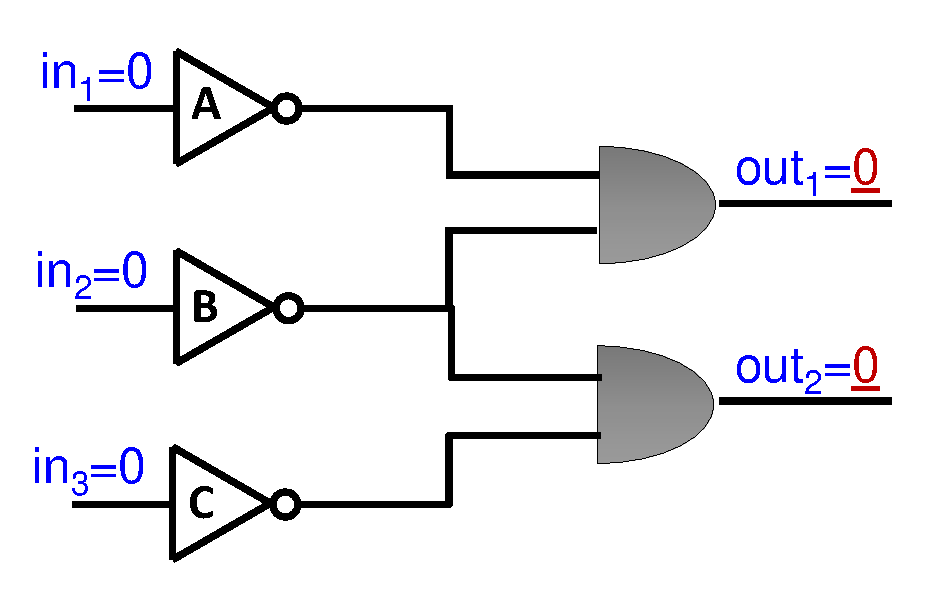
\includegraphics[width=0.5\columnwidth]{transition-example.pdf}%
\caption{An example to demonstrate the MDP transition functions used by \planbased .} %Assume that $p(\{B\})$=0.4, $p(\{B,A\})$=$p(\{B,C\})$=$p(\{A,C\})$=0.2. The possible system outputs after repairing $B$ would be $(0,0),(0,1),(1,0)$, $(1,1)$ with probability 0.2,0.2,0.2, and 0.4, respectively. The possible system outputs after repairing $A$ and $C$ would be $(0,0)$ and $(1,1)$ with probability 0.8 and 0.2, respectively.}
\vspace{-0.6cm}
\label{fig:transition-example}%
\end{center}
\end{figure}
%\end{wrapfigure}

% Example where several diagnoses have yield different observations
To demonstrate how the transition function is computed, consider the system described in Figure~\ref{fig:transition-example}. It is a logical circuit with outputs $(out_1,out_2)$ having an observed value of $(0,0)$ while the expected value is $(1,1)$. Assume that the diagnoses in $\Omega$ are $\{\{B\},\{B,A\},\{B,C\},\{A,C\}\}$, each with an abnormal behavior of flipping the value of its output, and the likelihoods of these diagnoses are 0.4, 0.2, 0.2, and 0.2, respectively\footnote{A diagnosis in $\Omega$ can be a subset of another diagnosis in $\Omega$.}. Consider the transition function for the possible outcomes of repairing $B$.
With 0.4 probability, the system is fixed.
With 0.2 probability, the correct diagnosis is $\{B,A\}$ and thus after fixing $\{B\}$ the system output would be $(0,1)$.
Similarly, there is a 0.2 probability to that the system output after repairing $\{B\}$ would be $(1,0)$ (for the case where the correct diagnosis is $\{B,C\}$),
and 0.2 probability for the system output to be $(0,0)$ (for the case where the correct diagnosis is $\{A,C\}$). Thus, repairing $B$ can lead to each of these 4 outcomes, and correspondingly to different MDP states.

% Example where several diagnoses have the same observations
Considering next the transition function for the possible outcomes of repairing $A$ and $C$. There is 0.2 probability that $\{A,C\}$ is the diagnosis, and subsets of $\{A,C\}$ are not diagnoses. Thus, there is a 0.2 probability for the system to be fixed. However, there is a 0.8 probability of observing $(0,0)$ after fixing $A$ and $C$, leading to the same MDP state for each of the remaining diagnoses  ($\{B\},\{B,A\},\{B,C\}$).


% What is a solution
A solution to an MDP is a policy, mapping every state to an action. In BRP, a policy maps every state reachable during the repair process to a repair action. We call such a policy a {\em repair policy}.

% Optimal solver
One can theoretically obtain an optimal repair policy by computing the optimal solution to the MDP above. There are several MDP solvers that return optimal solutions, such as value iteration, policy iteration~\cite{russell2010artificialIntelligence}, and LAO*~\cite{hansen2001lao}.
This would define the best repair action for every state reached during the repair process, where best means the repair action that minimizes the expected cost. We call this approach Optimal-BRP.

\subsection{State Space Size}
The state space of the MDP solved by Optimal-BRP is in practice too large to be solved optimally. First, the set of possible actions in a state is exponential in $|\overline{Repaired}|$, as every subset of $\overline{Repaired}$ can be a repair action. %[[Roni: footnote: can do operator decomposition to reduce branching factor at the cost of solution depth]]
Second, the number of states that can be reached after applying an action is also potentially exponential in the number of system outputs. This is because when a repair action fails, the set of possible observations is potentially equal to the number of diagnoses that are not ``fixed'' by the past repair actions. The number of such diagnoses can be exponential in the number of system components, but the number of different outputs is at most exponential in the number of system outputs.
%[[Add an example of both cases. Where the $\#diagnoses < 2^{\#outputs}$ and the other way around.]]
The state space described by our MDP is thus too large to be optimally solved in practice.
%$\meir{why dont you say that the action space is also exponential $2^{|COMPS|}$}[[Roni: I do.]]


However, solving MDPs with very large state spaces is a rapidly growing research field, especially when relaxing the requirement for optimal solutions. MDPs of a substantially larger scale can be solved suboptimally using an off-the-shelf suboptimal MDP solver. There are many suboptimal MDP solvers, such as Monte Carlo Planning (MCP)~\cite{silver2010monte} and Real-Time Dynamic Programming~\cite{barto1995learning}, as well as simply running Value or Policy iteration with earlier stopping conditions.